\documentclass[aspectratio=169]{beamer}
%
% Choose how your presentation looks.
%
% For more themes, color themes and font themes, see:
% http://deic.uab.es/~iblanes/beamer_gallery/index_by_theme.html
%
\mode<presentation>
%{https://writelatex.s3.amazonaws.com/vpzdvfpgmtcs/page/20577db5fb5206cebb645db53626924bd7e5686f.jpeg}
  \usetheme{Frankfurt}      % or try Darmstadt, Madrid, Warsaw, ...
  \usecolortheme{beaver} % or try albatross, beaver, crane, ...
  \usefonttheme{default}  % or try serif, structurebold, ...
  \setbeamertemplate{navigation symbols}{}
  \setbeamertemplate{caption}[numbered]{}
\setbeamertemplate{footline}[frame number]

\usepackage[english]{babel}
\usepackage[utf8x]{inputenc}
\usepackage{hyperref}
\usepackage{graphicx}
\usepackage{moreverb}

\title[GetL_Presentation]{Grammaires et Langages : Présentation}
\author{Equipe Minizza - H4111}
\institute{INSA de Lyon}
\date{Mardi 1 Avril}

\begin{document}

\begin{frame}
\titlepage
\end{frame}

% Plan proposé :
%
% 1. 


\section{Structures de données}
\subsection{Diagramme de classes}
\begin{frame}{Diagramme de classes}
\begin{center}
 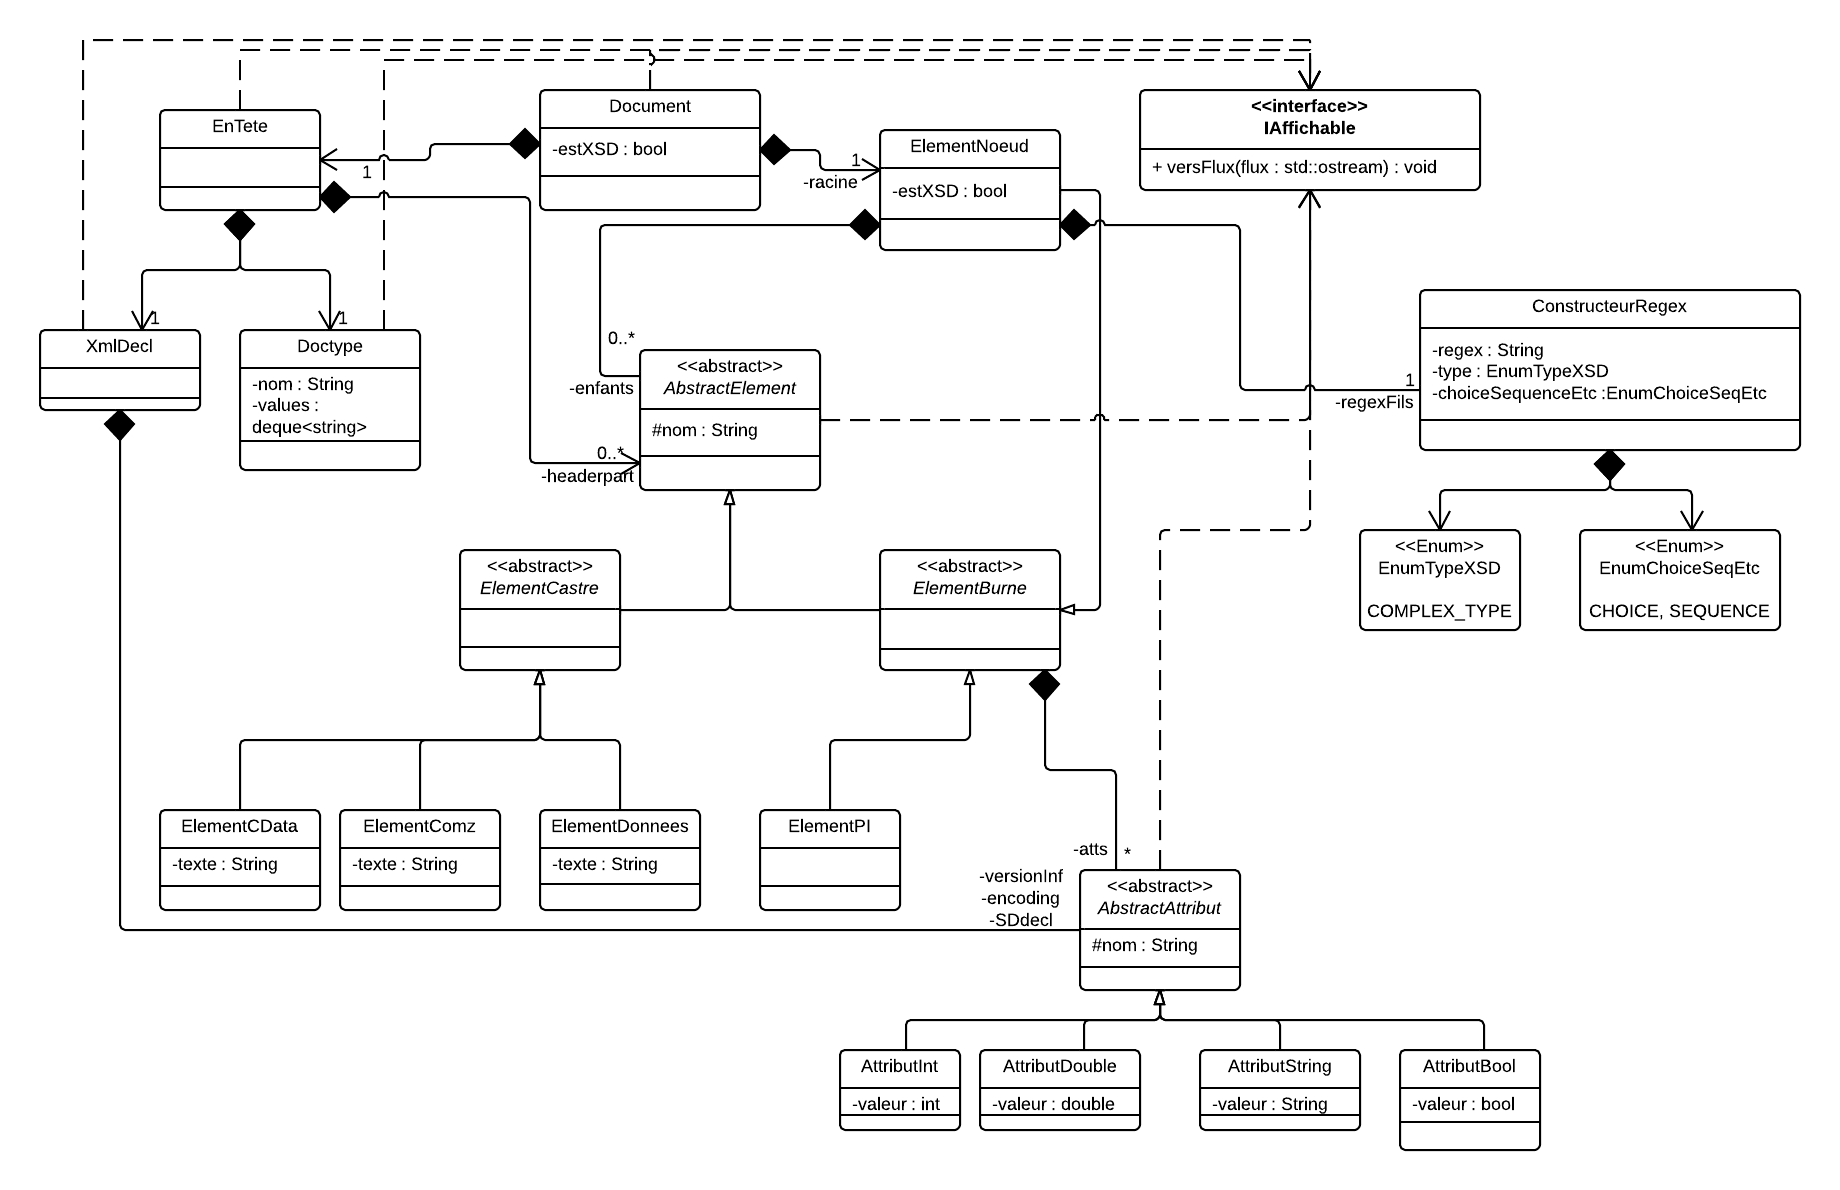
\includegraphics[scale=0.17]{diagdcla}
\end{center}
\end{frame}

\subsection{Diagramme de classes}
\begin{frame}{Diagramme de classes}
\begin{center}
  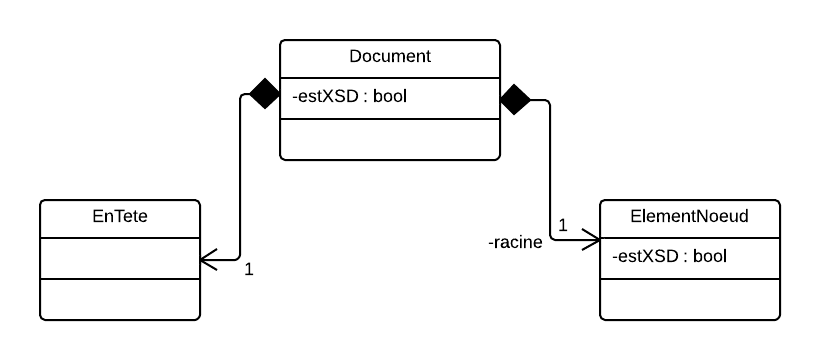
\includegraphics[scale=0.3]{ddc_doc}
\end{center}
\end{frame}

\subsection{Diagramme de classes}
\begin{frame}{Diagramme de classes}
\begin{center}
 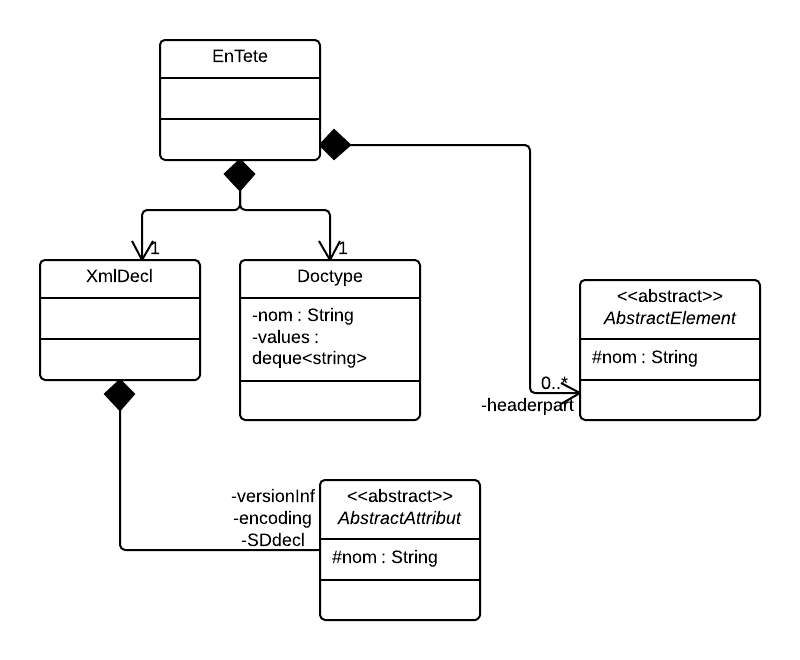
\includegraphics[scale=0.3]{ddc_ent}
\end{center}
\end{frame}

\subsection{Diagramme de classes}
\begin{frame}{Diagramme de classes}
\begin{center}
  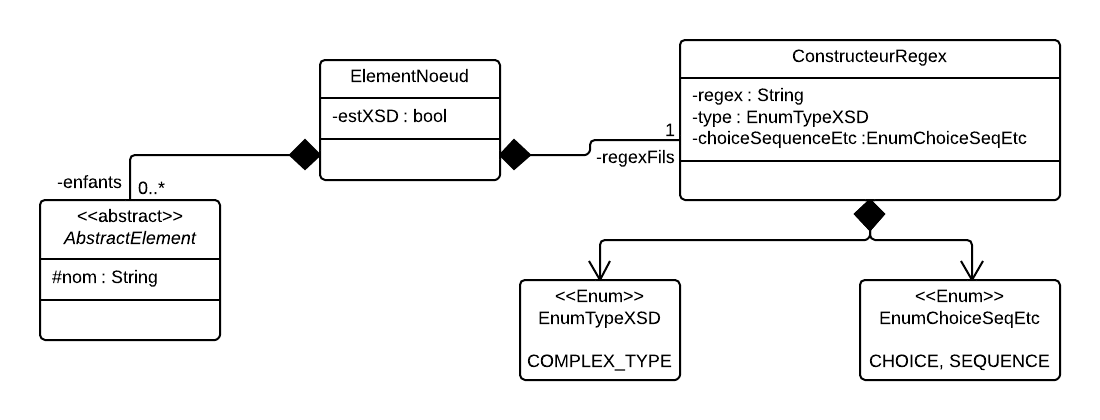
\includegraphics[scale=0.3]{ddc_noeud}
\end{center}
\end{frame}

\subsection{Diagramme de classes}
\begin{frame}{Diagramme de classes}
\begin{center}
  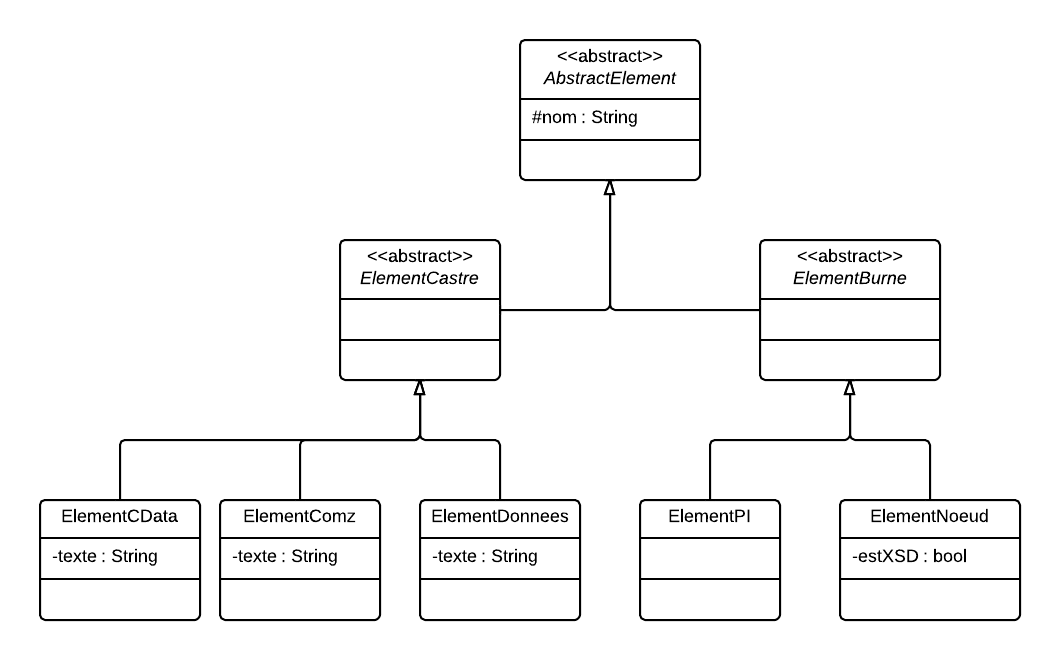
\includegraphics[scale=0.3]{ddc_abs_elmt}
\end{center}
\end{frame}

\subsection{Diagramme de classes}
\begin{frame}{Diagramme de classes}
\begin{center}
  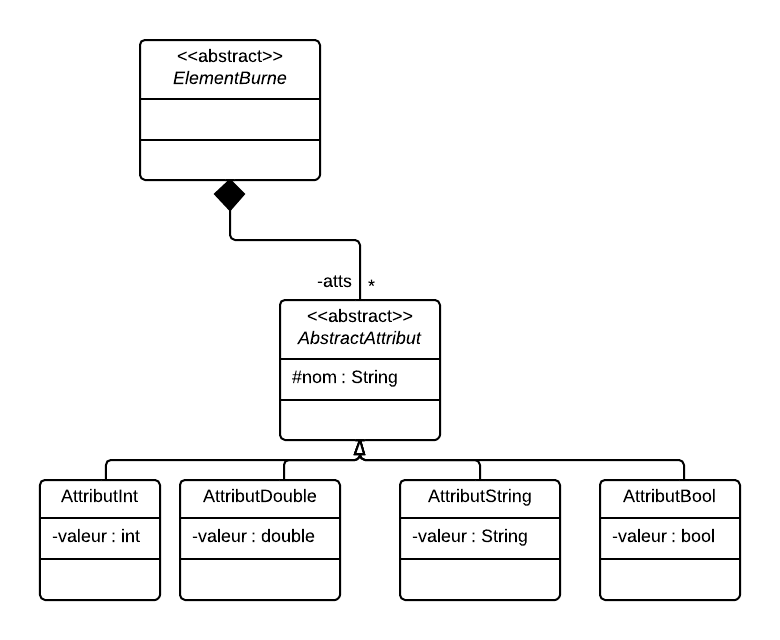
\includegraphics[scale=0.3]{ddc_elmt_burne}
\end{center}
\end{frame}

\subsection{Diagramme de classes}
\begin{frame}{Diagramme de classes}
\begin{center}
  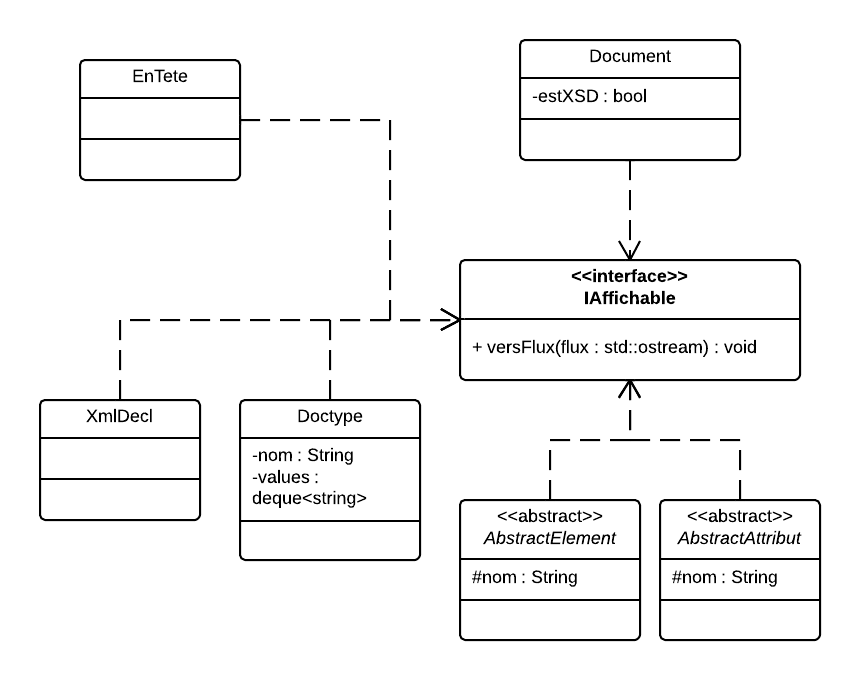
\includegraphics[scale=0.3]{ddc_iaff}
\end{center}
\end{frame}


\section{Algorithme de  validation}
\subsection{Algorithme de  validation}
\begin{frame}[fragile]{Algorithme de validation}
	\textbf{Objectif :}
	Cet algorithme permet de valider un document XML par rapport à un schéma XSD. \\
	\textbf{Principe :} algorithme en trois étapes :
	\begin{itemize}
		\item création d'un dictionnaire noeud/regex
		\item passage dans le dictionnaire pour traduire les références
		\item comparaison des regex avec la structure du document XML
	\end{itemize}
\end{frame}

\section{Algorithme de transformation}

\subsection{Algorithme de transformation}
\begin{frame}[fragile]{Algorithme de transformation - Fonctions Utiles }
	\textbf{Objectif :}
	Cet algorithme permet de transformer un document XML par rapport à une feuille de style XSL. \\
	\textbf{Principe :} 
	\begin{itemize}
		\item passage récursif dans chaque noeud du document XSL
		\item traitement en fonction du type de noeud
		\item sortie du résultat
\end{frame}

\section{Bilan du projet}
\subsection{Bilan quatitatif}
\begin{frame}{Bilan quantitatif}
\begin{center}
 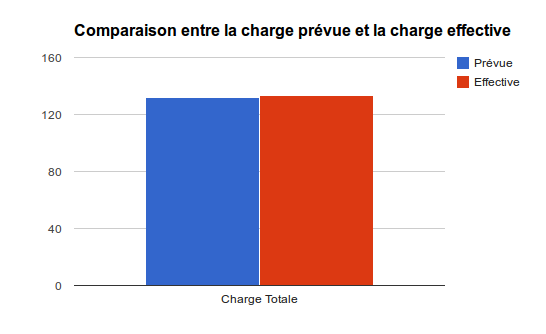
\includegraphics[scale=0.5]{chargetot}
\end{center}
\end{frame}

\subsection{Bilan quatitatif}
\begin{frame}{Bilan quantitatif}
\begin{center}
 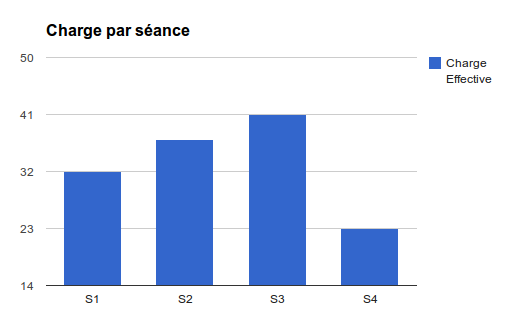
\includegraphics[scale=0.5]{chargeseance}
\end{center} 
\end{frame}

\subsection{Bilan quatitatif}
\begin{frame}{Bilan quantitatif}
 \begin{center}
 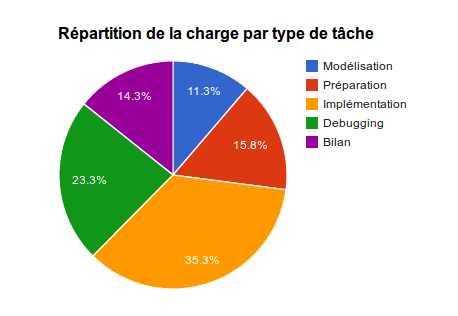
\includegraphics[scale=0.5]{chargetype}
\end{center}
\end{frame}

\subsection{Bilan qualitatif}
\begin{frame}{Bilan qualitatif}
Montées en compétence :
\begin{itemize}
 \item Modélisation pas évidente
 \item Développer la syntaxe
 \item Retoucher au C++
 \item Implémentation difficile
 \item Analyse des langages XML, XSD, XSL
\end{itemize}
\end{frame}

\subsection{Bilan qualitatif}
\begin{frame}{Bilan qualitatif}
Ressenti vis à vis du projet :
 \begin{itemize}
  \item Framework de test génial, très agréable
  \item Aucun souci avec ce qui nous a été donné
  \item Un projet bien dimensionné
  \item Un projet intéressant
 \end{itemize}
\end{frame}



\end{document}
